\documentclass[10pt,a4paper]{report}
\addtolength{\textheight}{-2cm}
\addtolength{\textwidth}{+2cm}
%------------------------------------------------------------------------------------------------------
\usepackage{xltxtra,fontspec,xunicode}
\usepackage[slantfont,boldfont]{xeCJK} % 允许斜体和粗体

\setCJKmainfont{WenQuanYi Micro Hei}             % 缺省中文字体
\setCJKmonofont{WenQuanYi Micro Hei Mono}        % 中文等宽字体
\setmainfont{DejaVu Serif}                       % 英文衬线字体
\setsansfont{DejaVu Sans}                        % 英文无衬线字体
\setmonofont{Monaco}                             % 英文等宽字体
%-------------------------------------------------------------------------------------------------------
\linespread{1.3}                                 % 1.5倍行距,值1.6产生双倍行距
% \setlength{\parindent}{0pt}                    % 段落首行缩进
\setlength{\parskip}{1ex plus 0.5ex minus 0.2ex} % 段落间距为1ex,可让TeX在+0.5到-0.8范围内微调
                                                 % 即实际范围在0.8ex~1.5ex之间
%-------------------------------------------------------------------------------------------------------
% 页眉与页脚设置
\usepackage{fancyhdr}
\pagestyle{fancy}
\fancyhf{}                                       %清空页眉页脚
\fancyhead[LE,RO]{\thepage}                      %页眉偶数页左,奇数页右
\fancyhead[RE]{\leftmark}                        %页眉偶数页右
\fancyhead[LO]{\rightmark}                       %页眉奇数页左
% \fancyfoot[LE,RO]{\thepage}                    %页脚偶数页左,奇数页右
% \fancyfoot[RE]{\leftmark}                      %页脚偶数页右
% \fancyfoot[LO]{\rightmark}                     %页脚奇数页左
\fancypagestyle{plain}{                          %重定义plain页面样式
    \fancyhf{}
    \renewcommand{\headrulewidth}{0pt}
}
%-------------------------------------------------------------------------------------------------------
% listings 与 xcolor 配合实现源代码的语法高亮
\usepackage{xcolor}
\usepackage{listings}
\lstset{
	language=Python,
	frame = shadowbox,
	basicstyle = \ttfamily\small,
	columns = fixed,
	numbers = left,
	numberstyle = \footnotesize,
	stepnumber = 1,
	tabsize = 2,
	showspaces = false,
	showstringspaces = false,
	showtabs = false,
	captionpos = b,
	breaklines = tr[],
	breakatwhitespace = false,
	backgroundcolor = \color{white},
	keywordstyle=\color{blue},
	numberstyle=\color[RGB]{0,192,192},
	commentstyle=\color[RGB]{0,96,96},
	stringstyle=\ttfamily\slshape\color[RGB]{128,0,0},
	escapeinside=``
}
%-------------------------------------------------------------------------------------------------------
\usepackage{graphicx}                            % 引入图片
\graphicspath{{img/}{images/}}                   % 要导入的图片的位置。可以有多个目录,但就算只有一个目录,也要用两级花括号
%-------------------------------------------------------------------------------------------------------
	\title{Python2.5学习笔记}                             % 文章的标题
	\author{                                     % 作者与致谢
		阿左 \thanks{感谢读者} \and 
		Nobody \thanks{感谢国家}
	}
	\date{\today}                                % 日期
	
%-------------------------------------------------------------------------------------------------------
\begin{document}
	\maketitle                                   % 制作标题
	\tableofcontents                             % 生成章节目录
	\setcounter{tocdepth}{5}                     % 生成章节的目录深度
	\listoffigures                               % 生成图片目录
	\listoftables                                % 生成表格目录


	\begin{abstract}                             % 英文摘要
		The Zen of Python, by Tim Peters

		Beautiful is better than ugly.

		Explicit is better than implicit.

		Simple is better than complex.

		Complex is better than complicated.

		Flat is better than nested.

		Sparse is better than dense.

		Readability counts.

		Special cases aren't special enough to break the rules.

		Although practicality beats purity.

		Errors should never pass silently.

		Unless explicitly silenced.

		In the face of ambiguity, refuse the temptation to guess.

		There should be one-- and preferably only one --obvious way to do it.

		Although that way may not be obvious at first unless you're Dutch.

		Now is better than never.

		Although never is often better than *right* now.

		If the implementation is hard to explain, it's a bad idea.

		If the implementation is easy to explain, it may be a good idea.

		Namespaces are one honking great idea -- let's do more of those!
	\end{abstract}

	\renewcommand{\abstractname}{摘要}           % 中文摘要
	\begin{abstract}

		Python之禅

		优美胜于丑陋,明了胜于晦涩;
		简洁胜于复杂,复杂胜于凌乱;
		扁平胜于嵌套,错落有致胜于密密匝匝。
		可读性不容轻视。

		即便觉得应该为实用性而放弃简单纯粹的时候,
		“存在特例”也不能成为违反上述规则的借口。

		不要让任何错误悄悄溜过,
		除非你确定不想让人看到报错。
		当存在多种可能时不要冒险猜测,
		尽量找到那唯一且明确的答案。

		虽然这在一开始并不容易,
		毕竟你不是Python之父。

		做也许好过不做,但不假思索就动手还不如不做。
		难以理解的实现方式绝对糟糕;
		简章易懂的实现方式往往不错。
		命名空间是一种绝妙的理念,让我们多加利用!
	\end{abstract}

	\part{语法基础}
		
\chapter{模块}

\section{模块与路径}

在linux环境下查找python的安装目录:

\begin{lstlisting}
whereis python
\end{lstlisting}

在python交互环境中查看python路径:

\begin{lstlisting}
sys.path
\end{lstlisting}

\section{导入模块}

\subsection{导入模块}

导入模块使用\verb|import|语句:

\begin{lstlisting}
import module01
\end{lstlisting}

当模块被导入后,会包含源文件的目录信息:<目录>/<文件名>.<扩展名>。

\subsection{重新导入模块}

一个模块只能有一个实例,导入一个模块以后不能再次导入。当一个模块的代码被修改以后必须使用\verb|reload|语句重新加载模块才能生效:

\begin{lstlisting}
reload module01
\end{lstlisting}

\verb|reload|只会重新导入写出的那个模块,不会自动导入相关的模块。

\subsection{部分导入模块}
如果只导入模块中的部分变量,则使用\verb|from|语句:

\begin{lstlisting}
from module01 import a, b, c
\end{lstlisting}

\verb|from|语句不导入模块,只复制模块中的变量到本地。复制模块中全部变量的例子:

\begin{lstlisting}
from module01 import *
\end{lstlisting}

\verb|import|与\verb|from|语句都都有赋值效果,例如:

\begin{lstlisting}
from module1 import a, b, c
\end{lstlisting}

等价于:

\begin{lstlisting}
import module1

a = module1.a
b = module1.b
c = module1.c
\end{lstlisting}

\subsection{防止变量被from复制}

方法一:下划线开头的变量不会被复制,如:“\verb|_X|”。

方法二:在顶层变量“\verb|__all__|”列表中的成员不会被复制出。如:

\begin{lstlisting}
__all__ = ['Error', 'encode']
\end{lstlisting}

\subsection{模块别名}

导入了模块以后,使用时要加上包名,所以有必要使用简写:

\begin{lstlisting}
import longname as name
\end{lstlisting}

等价于:

\begin{lstlisting}
import longname
name = longname
del longname
\end{lstlisting}

\verb|from|语句也可以用简写:

\begin{lstlisting}
from mod import longnmae as name
\end{lstlisting}

\subsection{判断是否是直接执行}

模块有\verb|__name__|属性。如果是被导入的,值为模块的名字;如果是被直接调用的,值为:\verb|'__main__'|。可以通过它判断程序是否是被导入的:

\begin{lstlisting}
if __name__ =  '__main__' :
	# in main
\end{lstlisting}

\section{直接执行脚本文件}

可以不加载模块而是直接以脚本文件的方式执行:

\begin{lstlisting}
execfile('mymodule.py')
\end{lstlisting}

\section{包的使用}

\subsection{建立自己的包}

包放在python检索的目录下。包目录与包下的每一级都要有\verb|__init__.py|文件(内容可以为空)表明这是一个包,\verb|__init__.py|文件中的语句都会在导入时被执行。例:

\begin{lstlisting}
# dir1/__init__.py
print 'dir1'
x = 1
\end{lstlisting}

\begin{lstlisting}
# dir1/dir2/__init__.py
print 'dir2'
y = 2
\end{lstlisting}

\begin{lstlisting}
# dir1/dir2/mod.py
print 'mod.py'
z = 3
\end{lstlisting}

\subsection{使用自己的包}

导入自己包的例子:

\begin{lstlisting}
% python
>>> import dir1.dir2.mod
dir1
dir2
mod.py

>>> import dir1.dir2.mod

>>> reload(dir1)
dir1

>>> reload(dir1.dir2)
dir2

>>> dir1.x
1
>>> dir1.dir2.y
2
>>> dir1.dir2.mod.z
3
\end{lstlisting}


		

\chapter{核心数据类型}

	在python的核数据类型中,数字、字符串、元组这三个对象是不可变的。

	\section{基本数字类型}
		
		数字对象是不可变的,许多对它的操作会生成一个新的对象返回,而不是改变原来的对象。

		\begin{verbatim}
			123, 5, 0                       # 同C语言的长整数
			999999999999L                   # 无限制长度
			1.23, 3.14e-10, 4E210, 4.0e+210 # 浮点数类似C语言双精度数
			0177, 0x13e, 0X3e               # 八进制与十六进制
			3+4j, 3.0+4.0j, 3J              # 复数,实数加上复数
		\end{verbatim}

		格式化数字:

		\lstinputlisting[firstline=1,lastline=7]{py/coreda/exnum.py}

		常用操作:加(\verb|+|)、减(\verb|-|)、乘(\verb|*|)、除(\verb|/|)、下取整(\verb|//|)、乘方(\verb|**|)、位移(\verb|>>|)等:

		\lstinputlisting[firstline=9,lastline=16]{py/coreda/exnum.py}

		调用内置的函数进行强制类型转换:

		\lstinputlisting[firstline=18,lastline=27]{py/coreda/exnum.py}

		\subsection{常用数学模块}

		\lstinputlisting{py/coreda/exmatch.py}

	\section{十进制小数类型}

		集合类型set可以支持一般的数学集合操作:

		\lstinputlisting{py/coreda/exdecimal.py}

	\section{序列类型的共同点}
		
		字符串、列表、元组都属于序列类型类型,会支持一些共同的操作。

		索引操作:

		\lstinputlisting[firstline=1,lastline=10]{py/coreda/exstr.py}

		分片操作:
		\lstinputlisting[firstline=11,lastline=17]{py/coreda/exstr.py}

		连接与重复操作会生成新的对象:
		\lstinputlisting[firstline=19,lastline=20]{py/coreda/exstr.py}

	\section{字符串类型}

		字符串也是一种序列类型,所以支持所有的序列操作。

		字符串对象是不可变的,许多对它的操作会生成一个新的对象返回,而不是改变原来的对象。

		\lstinputlisting[firstline=22,lastline=32]{py/coreda/exstr.py}

	\section{列表}

		列表也是一种序列类型,所以支持所有的序列操作。

		虽然列表没有固定大小,但是还是会越界。越界会抛出IndexError。
		
		列表常用的特定操作:

		\lstinputlisting[firstline=1,lastline=11]{py/coreda/exlist.py}

		列表可以进行嵌套,并且经常被用在多维数组上:

		\lstinputlisting[firstline=13,lastline=26]{py/coreda/exlist.py}

	\section{字典}

		不能读取一个字典中不存在的键:

		\lstinputlisting[firstline=1,lastline=25]{py/coreda/exdict.py}

		对字典内容进行排序:

		\lstinputlisting[firstline=27,lastline=35]{py/coreda/exdict.py}

	\section{元组}

		元组也是一种序列类型,所以支持所有的序列操作。

		元组对象是不可变的,许多对它的操作会生成一个新的对象返回,而不是改变原来的对象。

		\lstinputlisting[firstline=1,lastline=12]{py/coreda/exfile.py}
		
	\section{集合类型}

		集合类型set可以支持一般的数学集合操作:

		\lstinputlisting{py/coreda/exset.py}
		
	\section{bool类型与空}

		bool类型实际是在以定制后的逻辑来显示整数的1和0。

		None对象表示空
		
		\lstinputlisting{py/coreda/exbool.py}

	\section{type类型}

		再次强调python中的类型信息与变量无关,类型是关联在对象上的。

		\lstinputlisting{py/coreda/extype.py}


		
\chapter{语句顺序}

	\section{if语句}

		基本结构:
		
\begin{lstlisting}
if ... :
	...
elif ... :
	...
else
	...
\end{lstlisting}

		\subsection{推荐风格}

			对于过长的语句可以使用“\verb|\|”换行:

\begin{lstlisting}
if a==b and b==c \
	 and c==d :
	 print 'all equal!'
\end{lstlisting}

			但推荐还是用“\verb|()|”包起来在风格上更好:

\begin{lstlisting}
if (a==b and b==c
	 and c==d):
	 print 'all equal!'
\end{lstlisting}

	\section{三元表达式}

\begin{lstlisting}
<normal> if <condition> else <other>
\end{lstlisting}
	

	\section{用字典实现判断}

		python中的字典也可以部分实现if-else的功能。因为字典不但可以用函数作为成员,而且取值操作时,可以指定找不到值的默认返回值:

\begin{lstlisting}
myDict.get('aaa','no value');  # default value if key not exist
\end{lstlisting}

	\section{while循环语句}

\begin{lstlisting}
while ... :
	...      # 执行的语句
	...      # 遇到 break 跳出整个循环
	...      # 遇到 continue 回到开头进行
	...      # pass 语句什么也不做,仅在语法上点一个位置
else :
	...      # 只有在循环完全执行后才会运行(没有遇到break)
\end{lstlisting}

	\section{for循环语句}

\begin{lstlisting}
for ... in ... :
	...      # 执行的语句
	...      # 遇到 break 跳出整个循环
	...      # 遇到 continue 回到开头进行
	...      # pass 语句什么也不做,仅在语法上点一个位置
else :
	...      # 只有在循环完全执行后才会运行(没有遇到break)
\end{lstlisting}
		
		\subsection{for循环例子}

			用\verb|xreadlines()|一行一行地读入文本文件,防止文件过大:

\begin{lstlisting}
for line in open('log.txt').xreadlines():
	print line
\end{lstlisting}

			用推荐自动用速度快而内存利用最合理的方法:

\begin{lstlisting}
for line in open('log.txt'):
	print line
\end{lstlisting}

			用\verb|range()|函数生成列表的方法:

\begin{lstlisting}
range(5)        # [0,1,2,3,4]
range(2, 5)     # [2,3,4]
range(0, 10, 2) # [0,2,4,6,8]
\end{lstlisting}

			结合\verb|range()|函数与for循环:

\begin{lstlisting}
for x in range(5, -5, 2):
	print x

for i in range(len('abc')):
	print 'abc'[i]
\end{lstlisting}

	\section{迭代器}

		\subsection{通用迭代器}

			python中所有的对象都可以被迭代,迭代的工具是通用迭代器\verb|next()|。当没有可迭代的项时接收\verb|StopIteration|异常决定离开。

		\subsection{文件迭代}

			文件迭代可以使用包装过了\verb|reanline()|。它会的文件结尾返回空字符串\verb|''|:

\begin{lstlisting}
file = open('log.txt')
file.readline()
file.readline()
file.readline()
...
file.readline()        # return '' at end of file
\end{lstlisting}

		\subsection{常见的迭代器用法}

			处理每个成员
\begin{lstlisting}
list = [line.upper() for line in lines]
\end{lstlisting}

			map()函数,声明用指定的方法处理每个成员

\begin{lstlisting}
map(str.upper, lines)         
\end{lstlisting}

			成员处理

\begin{lstlisting}
'3' in lines      # 是否包含成员
sort(lines)
sum([1,2,3,4,5])
any(['a','','c'])
all(['a','','c'])
\end{lstlisting}

			转换类函数

\begin{lstlisting}
list(line)        # 转为列表
tuple(line)       # 转为元组
\end{lstlisting}

			合并多个可迭代序列

\begin{lstlisting}
zip('ABC','abc','123') 
# result (('A','a','1'), ('B','b','2'), ('C','c','3'))
\end{lstlisting}

			enumerate()把列表解析为“下标”与“值”的形式

\begin{lstlisting}
items = enumerate('abc')
items.next()             # result is (0,'a')
\end{lstlisting}

			结合enumerate()与for循环

\begin{lstlisting}
for (index, value) in enumerate('abc')
\end{lstlisting}

	\section{列表解析}

		列表解析以中括号围起的单行for循环的形式编写:

\begin{lstlisting}
[... for ... in ...]
\end{lstlisting}

		一般来说,列表解析会比用for循环更快。原因是在底层有优化,它是以C运行的。在速度上“列表解析”快于“map”快于“for循环”。

		\subsection{列表解析与for循环结合的例子}
			
			读取文件并且去除最后的换行符:

\begin{lstlisting}
lines = [line.rstrip() for line in open('log.txt')]
\end{lstlisting}

			组合for与if读取以“p”开头的行:

\begin{lstlisting}
lines = [line.rstrip() for line in open('log.txt') if line[0]=='p'] 
\end{lstlisting}

			列表解析也可以嵌套:

\begin{lstlisting}
[x+y for x in 'abc' for y in '123']
# result is ['a1','a2','a3' ... 'c1','c2','c3']
\end{lstlisting}

			列表解析与多维数组结合:

			\lstinputlisting[firstline=13,lastline=26]{py/coreda/exlist.py}


		
\chapter{函数}

	\section{函数定义}

		python中,函数也是一个对象。\verb|def|语句定义一个函数对象,然后赋值给指定函数名变量:

\begin{lstlisting}
def myAdd(a, b):
	return a+b
\end{lstlisting}

		以上代码生成了一个函数对象,并且把这个对象赋值给了变量\verb|myAdd|。可以通过变量\verb|myAdd|调用这个函数:

\begin{lstlisting}
myAdd(1,2)
\end{lstlisting}

		也可以把函数再赋值给另一个变量:

\begin{lstlisting}
otherFunc = myadd
otherFunc(1,2)
\end{lstlisting}

		函数对象的生成与赋值是在运行时发生的。所以也可以在运行时创建函数:

\begin{lstlisting}
if a>3:
	otherFunc = funcA
if a<3:
	otherFunc = funcB
\end{lstlisting}
		
	\section{参数传递}

		函数参数没有参数类型限制,只要参数支持对应的操作就可以。如果参数不支持对应的操作会抛出异常。

		函数参数列表支持\verb|name=value|形式的默认值:

\begin{lstlisting}
def myAdd(a=1, b=2):
	return a+b
\end{lstlisting}

		函数的默认参数被认为是静态的,不会每次调用都生成一个新的对象。

		函数都有返回值。没有return或yield语句的函数会返回一个None。

		\subsection{参数传递}
			python支持可变参数。当定义函数时,\verb|*|表示列表、\verb|**|表示字典:

\begin{lstlisting}
def func(a, * pargs, ** kargs):
    print a, pargs, kargs

func(1,2,3,x=1,y=2)           # 1 (2, 3) {'y': 2, 'x': 1}
\end{lstlisting}

			当调用函数时,\verb|*|表示把列表打散成多个参数、\verb|**|表示把字典打散作为参数:
\begin{lstlisting}
lst = (1,2,3,4,5)
dic = {'a':1,'b':2,'c':3}

func(*lst)                    # 1 (2, 3, 4, 5) {}
func(**dic)                   # 1 () {'c': 3, 'b': 2}

def func(a,b,c):
	print a

func( *(1,2,3) )         # OK
func(  (1,2,3) )          # err
func(  2 )                # err
\end{lstlisting}

			混合使用参数的格式:

\begin{lstlisting}
def func(a,b,c,... j=k,l=m,... *p,*q,... **x,**y...)
         ^         ^           ^         ^
         normal    key-value   seq       dict
\end{lstlisting}

	\section{lambda表达式}

		lambda表达式中不能出现语句,只能用表达式。例:

\begin{lstlisting}
f = lambda a,b : a+b
f(1,2)
\end{lstlisting}

		用表达式替代常用语句。例:

\begin{lstlisting}
lbd = lambda x : sys.stdout.write(x+'\n')
lbd('aaa')

lbd = lambda x : map(sys.stdout.write, x)
lbd(['aaa\n','bbb\n','ccc\n'])

lbd = lambda x : [sys.stdout.write(line) for line in x]
lbd(['aaa\n','bbb\n','ccc\n'])
\end{lstlisting}

	\section{闭包}

		一个函数的成员变量可以被定义在这个函数内部的内部函数访问。

		在早期不支持闭包的版本中,内部函数不能访问外部函数的变量;只能通过参数的默认值来取得外部函数变量的值:

\begin{lstlisting}
def func1():
	x = 88
	def func2(x=x):
		print x
	func2()
\end{lstlisting}

		在使用闭包的情况下:

\begin{lstlisting}
def func1():
	x = 88
	def func2():
		print x
	return func2

action = func1() # call func1()
action()         # call func2()
\end{lstlisting}

		要注意的一点是:函数只有在第一次被调用时存在。
		
		所以下面的例子中,变量\verb|i|的值永远是4。而不是随循环从0增长到4:

\begin{lstlisting}
def func1():
	acts = []
	for i in range(5):
		acts.append(lambda x: i ** x)
	return acts
\end{lstlisting}

		在这种情况下,只能使用默认参数:

\begin{lstlisting}
def func1():
	acts = []
	for i in range(5):
		acts.append(lambda x,i=i: i ** x)
	return acts
\end{lstlisting}



		\取chapter{OOP与类}

一个模块只能有一个实例,当一个模块的代码被修改以后必须重新加载模块才能生效;类可以同时创建多个实例(即对象)。

\section{最简单的Python类}

Python的类模型相当动态,类与实例只是命名空间对象。

可以仅用pass作为占位语句生成一个没有任何成员的class,这样的class仅仅是一个空的命名空间对象。可以在以后通过赋值给这个类加上新的成员:

\begin{lstlisting}
class C1: pass             # Empty class
                           # as an namespace object

a = C1()
a.name = "morgan"          # a.name is "morgan"

C1.name = "Class C1"       # C1.name is "C1"
b = C1()                   # b.name is "C1"
                           # a.name still is "morgan"

def upperName(self):
	print self.name.upper()

C1.showName = upperName    # add func to class
a.showName()
b.showName()
\end{lstlisting}

\section{类与实例的基本概念}

类与类的实例都是对象。类是一个对象,该类的每个实例又各对应了一个关联到该类对象的实例对象。

像调用函数一样调用类对象会创建该类的实例对象。每个实例对象根据具体类的创建属性并获得自己的命名空间,每个成员都有自己的实例。

对象的数据成员(无论是数据还是函数)在没有被第一次赋值之前,都不能被访问(就像是没有被声明的变量一样)。同样地也可以简章地通过赋值给变量增加一个成员。

class语句会创建一个类对象并赋值给变量名。class语句块内的语句会创建数据对象和方法对象赋值给类的成员变量。类的成员变成只属于该类,不属于该类的实例,但可以被所有的实例共享访问。

\begin{lstlisting}
class Ca:
	v = 42

a = Ca()   # a.v = 42
b = Ca()   # b.v = 42

Ca.v = 55  # Ca.v = 55
           # a.v = 55
		   # b.v = 55

a.v = 11   # Ca.v = 55
           # a.v = 11
		   # b.v = 55
\end{lstlisting}

类中的方法被所有函数共享。通过实例调用方法时,会把这个实例对象作为第一个参数self传递给方法。


wwwgwgwgbwgbwgbbwgbb例子:

class c1():
	count = 0
	def show(self):
		print 'c1.show()'
\end{lstlisting}

类的构造函数是\verb|__init__|;析构函数是\verb|__del__|:

\begin{lstlisting}
class Life:
	def __init__(self, name='unknow'):
		print 'hello ', name
		self.name = name
	def __del__(self):
		print 'goodbye ', self.name

brian = Life('Brian')     # prints: hello Brian
brian = 'loretta'         # prints: goodbye Brian
\end{lstlisting}

		实例对象的\verb|__class__|属性记录了这个实例的类对象。

\begin{lstlisting}
print a.__class__           # class of instance
\end{lstlisting}

\section{类的成员}

\subsection{属性与方法}

python中对于类和对象,无论数据还是方法都作为变量处理。对象的数据成员(无论是数据还是函数)在没有被第一次赋值之前,都不能被访问(就像是没有被声明的变量一样)。同样地也可以简单地通过赋值给变量增加一个成员。

\begin{lstlisting}
class Employee():
	def __init__(self, name):   # __init__ defing construter
		self.name = name
	def showName(self):
		print self.name

morgan = Employee("Morgan")
morgan.showName()

morgan.showName = "new name"    # set value
morgan.nickName = "Jade"        # create new variable
\end{lstlisting}

类对象与实例对象的\verb|__dict__|属性是大多数基于类的对象的命名空间字典。

\begin{lstlisting}
print Employee.__dict__.keys()  # 大多数基于类的对象的命名空间字典
print morgan.__dict__.keys()    # 大多数基于类的对象的命名空间字典
\end{lstlisting}

\subsection{类属性与对象属性}

修改了类的属性以后会影响到所有的类实例:

\begin{lstlisting}
class C:
	a = 1

print C.a     # is 1
o = C()
print o.a     # is 1

C.a = 2
print o.a    # is 2, also change too

j = X()
print j.a   # is 2
\end{lstlisting}

\subsection{方法与对象的绑定}

对于以下的类:

\begin{lstlisting}
class Spam:
	def doit(self, message):
		print message
\end{lstlisting}

可以通过新建对象调用:

\begin{lstlisting}
obj = Spam()
obj.doit('hello world')
\end{lstlisting}

已经绑定的方法可以再赋值给一个变量,效果和对象点号调用一样:

\begin{lstlisting}
x = obj.doit
x('hello world')
\end{lstlisting}

但是类中的方法是没有绑定到对象的,要传入对象:

\begin{lstlisting}
t = Spam.doit
t(obj, 'hello world')
\end{lstlisting}

同理,如果要引致类中的函数,相同的规则也适用于类的方法:

\begin{lstlisting}
class Eggs:
	def m1(self, n):
		print n

	def m2(self):
		x = self.m1  # bound to object
		x(42)

Eggs().m2()
\end{lstlisting}

\section{类的继承}

类对象的成员\verb|__bases__|是超类构成的元组

\begin{lstlisting}
print c3.__bases__              # 超类的元组
\end{lstlisting}

通过\verb|Super|调用超类:

\begin{lstlisting}
class Super:
	def __init__(self):
		pass

class Sub(Super):
	def __init__(self):
		Super.__init__(self):
			pass
\end{lstlisting}

\subsection{多重继承}

子类会继承父类的成员。如果当多重继承时遇到重名成员时顺序就很重要,优先级按声明继承时从左到右顺序:

\begin{lstlisting}
class c1():
	myname = 'aaa'
	def show(self):
		print 'c1.show()'
	def helloC1(self):
		print 'c1.helloC1()'

class c2():
	def show(self):
		print 'c2.show()'
	def helloC2(self):
		print 'c2.helloC2()'

class c3(c1, c2):               # 超类写在括号中,支持多重继承
	def show(self):
		print 'c3.show()'

c1.myname                       # c1.myname is 'aaa'
c3.myname                       # c3.myname is 'aaa'
\end{lstlisting}

对象成员赋值后不影响类成员的值:

\begin{lstlisting}
i1 = c3()                       # i1.myname is 'aaa'
i2 = c3()                       # i2.myname is 'aaa'

i1.myname = 'this is i1'        # i1.myname is 'this is i1'
i2.myname = 'this is i2'        # i2.myname is 'this is i2'
print c1.myname                 # c1.myname still is 'aaa'
print c3.myname                 # c3.myname still is 'aaa'

i1.show()                       # 调用重写的方法
i1.helloC1()                    # 调用到父类的方法
i1.helloC2()                    # 调用到父类的方法
\end{lstlisting}

虽然顺序很重要,但是也可以手动指定要调用哪一个:

\begin{lstlisting}
class A:
	def __repr__(self): pass
	def other(self): pass

class B:
	def __repr__(self): pass
	def other(self): pass

class C(A, B):
	__repr__ = A.__repr__
	other = B.other
\end{lstlisting}

\subsection{压缩成员变量名}

常见的变量名重复的情况:

\begin{lstlisting}
class C1:
	def meth1(self): self.x = 88
	def meth2(self): print self.x

class C2:
	def metha(self): self.x = 99
	def methb(self): print self.x

class C3(C1, C2): pass

I = C3()   # only 1 x in I !!!
\end{lstlisting}

在这样的情况下,x只有一个。两个类的四个方法读写的都是同一个x成员。这个x是值取决最后是哪一个方法调用的它。 

在\verb|__class__|语句中以两个下划线开头的变量\verb|__verb|会扩展成包含类名的新变量名\verb|_classname__verb|。这样就不会和同一层次中其他类所创建的类似变量名相冲突。

\begin{lstlisting}
class C1:
	def meth1(self): self.__x = 88
	def meth2(self): print self.__x

class C2:
	def metha(self): self.__x = 99
	def methb(self): print self.__x

class C3(C1, C2): pass

I = C3()   # two x in I: _C1__x and _C2__x

I.meth1()
I.meth2()  # result is 88

I.metha()
I.methb()  # result is 99
\end{lstlisting}


\subsection{继承的应用场景}

一般由超类提供默认的方法或是等待实现的方法:

\begin{lstlisting}
class Super:
	def method(self):
		print 'Super.method()'           # default behavior
	def delegate(self):
		self.action()                    # expected to defined
\end{lstlisting}

子类可以不去实现超类:

\begin{lstlisting}
class Inheritor(Super):
	pass                                 # inherit method verbatim
\end{lstlisting}

子类可以把超类的方法完全覆盖掉:

\begin{lstlisting}
class Replacer(Super):
	def method(self):
		print 'Replacer.method()'        # replace method completely
\end{lstlisting}

子类可以扩展超类的方法:

\begin{lstlisting}
class Extender(Super):
	def method(self):                    # extend method behavior
		print 'Extender.method() start'
		Super.method(self)
		print 'Extender.method() end'
\end{lstlisting}

子类可以实现超类有待实现的方法:
		
\begin{lstlisting}
class Provider(Super):                   # fill in required method
	def action(self):
		print 'Provider.action'
\end{lstlisting}

在迭代中创建类:

\begin{lstlisting}
if __name__ == '__main__':
	for clazz in (Inheritor, Replacer, Extender):
		print '\n' + clazz.__name__ + '...'
		clazz().method()
	print '\nProvider...'
	p = Provider()
	p.delegate()
\end{lstlisting}

\section{命名空间}

\subsection{命名空间范围}

python中作用域是由源代码中赋值语句位置来决定的,不会受到导入关系的影响。通过下面的例子总结了python的命名空间:

\lstinputlisting[]{py/chap.oop/manynames.py}

需要注意的是在调用I.m()之前实例中是不存在成员变量X的。实例的成员变量也是变量,在执行到赋值语句之前是不会存在的。

在外部文件中使用:

\lstinputlisting[]{py/chap.oop/otherfile.py}

\subsection{命名空间字典}

无论是模块、对象还是实例,它们的命名空间实际都是以字典形式实现的。这个字典就是对象中的成员\verb|__dict__|变量。

\begin{lstlisting}
>>> class super:
...     def hello(self):
...             self.data1 = 'spam'
... 
>>> class sub(super):
...     def hola(self):
...             self.data2 = 'eggs'
... 
>>> X = sub()
>>> X.__dict__
{}
>>> X.__class__
<class __main__.sub at 0x7f35b8248ef0>
>>> sub.__bases__
(<class __main__.super at 0x7f35b8248e88>,)
>>> super.__bases__
()
\end{lstlisting}

以\verb|self|为目标赋值会把成员加入到对象,而不是类中:

\begin{lstlisting}
>>> Y = sub()

>>> X.hello()
>>> X.__dict__
{'data1': 'spam'}

>>> X.hola()
>>> X.__dict__
{'data1': 'spam', 'data2': 'eggs'}

>>> sub.__dict__
{'__module__': '__main__', '__doc__': None, 'hola': <function hola at 0x7f35b8201668>}

>>> super.__dict__
{'__module__': '__main__', 'hello': <function hello at 0x7f35b82015f0>, '__doc__': None}

>>> Y.__dict__
{}
\end{lstlisting}

可以用命名空间字典部分实现点号操作,但是字典不带继承搜索:

\begin{lstlisting}
>>> X.__dict__['data1']
'spam'

>>> X.__dict__['data3'] = 'ham'
>>> X.data3
'ham'
\end{lstlisting}

\subsection{命名空间链接}

每个类的实例,都有成员变量\verb|__class__|连接到它的类;

而在类中有成员变量\verb|__bases__|是一个元组,包含了到超类的链接。

\section{运算符重载}

两头是双下划线的方法名(\verb|__方法名__|)表示对运算符的重载。

\subsection{重载字符串化方法}

当要把实例字符串化时会先使用\verb|__str__|。这样产生的结果在终端下用户体验较好; 如果没有定义,会再调用\verb|__repr__|,它产生的结果可以作为代码直接重建该对象。

\begin{lstlisting}
class adder:
	def __init__(self, value=0):
		self.data = value
	def __str__(self):
		return '[value is: %s]' % self.data
	def __repr__(self):
		return 'addrepr(%s)' % self.data

x = adder(2)
print x          # [value is: 2]
print str(x)     # [value is: 2]
print repr(x)    # addrepr(2)
\end{lstlisting}

\subsection{常用数学方法}

\verb|__add__|表示重载\verb|+|运算。

\verb|__sub__|表示重载\verb|-|运算。

\verb|__mul__|表示重载\verb|*|运算。

对于没有定义或是继承的操作符,表示该操作不被支持。

\begin{lstlisting}
class Number():
	def __init__(self, value):
		self.data = value
	def __add__(self, other):
		return C1(self.data + other)
	def __sub__(self, other):
		return C1(self.data - other)
	def __mul__(self, other):
		return C1(self.data * other)

a = Number(5)       # Number.__init__(a,5)
b = a - 2           # Number.__sub__(a,2)
\end{lstlisting}

以上的方法中,操作符右边的不能是实例对象。还有一个相反的左边不是对象右边是对象的\verb|__radd__|方法:

\begin{lstlisting}
class Computer:
	def __init__(self, val):
		self.val = val
	def __add__(self,other):
		self.val += other
	def __radd__(self, other):
		self.val = self.val + other

x = Computer(2)
x + 3
print x.val

y = Computer(3)
3 + y
print y.val
\end{lstlisting}

\subsection{拦截索引}

索引操作可以通过\verb|__getitem__|方法拦截:

\begin{lstlisting}
class indexer:
	def __getitem__(self,index):
		return index ** 2

x = indexer()
x[2]                      # __getitem__(x,2)  result 4
\end{lstlisting}

索引操作可以模拟迭代效果:

\begin{lstlisting}
class stepper:
	def __getitem__(self,index):
		return self.data[i]

x = stepper()
x.data = "spam"

for item in x:
	print item
\end{lstlisting}

\subsection{拦截迭代}

迭代操作可以通过\verb|__iter__|方法拦截,python在遇到迭代环境时会先尝试迭代,如果对象不支持迭代,就会尝试索引运算:

\begin{lstlisting}
class Squares:
	def __init__(self, start, stop):    # save state when created
		self.value = start -1
		self.stop = stop
	def __iter__(self):          # get iterator object on iter()
		return self
	def next(self):              # return a square on each iteration
		if self.value == self.stop:
			raise StopIteration
		self.value += 1
		return self.value ** 2

for i in Squares(1,5):   # for calls iter(), which calls __iter__()
	print i              # Each iteration calls next()
	                     # get result: 1 4 9 16 25
\end{lstlisting}

\verb|__iter__|只循环一次,循环以后就变为空,每次新的循环就必须重新创建一个新的迭代器对象。

\begin{lstlisting}
x = Squares(1,5)
[n for n in x]            # [1,4,9,16,25]
[n for n in x]            # [] now it's empty
[n for n in Squares(1,5)] # [1,4,9,16,25]
list(Squares(1,3))        # [1,4,9]
\end{lstlisting}

另外一个例子,迭代时跳过下一下元素:

\begin{lstlisting}
class SkipIterator:
	def __init__(self, wrapped):
		self.wrapped = wrapped  # iter state flg
		self.offset = 0
	def next(self):
		if self.offset >= len(self.wrapped):
			raise StopIteration
		else:
			item = self.wrapped[self.offset]
			self.offset += 2
			return item

class SkipObject:
	def __init__(self,wrapped):
		self.wrapped = wrapped
	def __iter__(self):
		return SkipIterator(self.wrapped)

if __name__ == '__main__':
	skipper = SkipObject('0123456789')
	i = iter(skipper)   # make an iterator on it
	print i.next(), i.next(), i.next()
	
	# in earch nest create new iterator
	for c in skipper:
		for d in skipper:
			print c+d
\end{lstlisting}

在最后的嵌套的两个\verb|for|循环中,每个循环都会建立自己的迭代器,相互之间不会混淆。这相的操作相当于:

\begin{lstlisting}
str = 'abcdefg'
for x in s[::2]
	for y in s[::2]
		print x+y
\end{lstlisting}

这里迭代与分片的区别是。分片把结果的整个列表放到了内存里,而迭代器每次产一个值;分片会产一个新的对象,并不同于迭代是对原来的对象进行r操作。

\subsection{拦截成员属性}

\verb|__getattr__|对成员属性的点号操作时行拦截(多数情况下是对没有定义的成员属性):

\begin{lstlisting}
class empty:
	height = 189
	def __getattr__(self,name):
		if attrname == "age":
			return 40

x.age          # 40
x.height       # 189
x.name         # None
\end{lstlisting}

其他属性抛出异常:

\begin{lstlisting}
class empty:
	height = 189
	def __getattr__(self,name):
		if attrname == "age":
			return 40
		else:
			raise AttributeError, attrname

x.age          # 40
x.height       # 189
x.name         # exception
\end{lstlisting}

\verb|__setattr__|对成员属性的赋值操作进行拦截。但有个问题:即使在\verb|__setattr__|内的\verb|self.attr=value|也会再次被拦截,造成无限循环。所以在拦截函数内要通过:\verb|self.__dict__['name']=value|来赋值:

\begin{lstlisting}
class AccessControl:
	def __setattr__(self,attr,value):
		if attr == 'age':
			self.__dict__[attr] = value
		else:
			raise AttributeError, attr + ' not allowed'

x = AccessControl()
x.age = 40
\end{lstlisting}

\subsection{模拟私有成员}

\begin{lstlisting}
class PrivateExc(Exception):pass

class Privacy:
	def __setattr__(self, attrname, value):
		if attrname in self.privates:
			raise PrivateExc(attrname, self)
		else:
			self.__dict__[attrname] = value

class Test1(Privacy):
	privates = ['age']

class Test2(Privacy):
	privates = ['name','pay']
	def __init__(self):
		self.__dict__['name'] = 'Tom'
\end{lstlisting}

\subsection{拦截调用}

如果定义了\verb|__call__|方法,实例的调用就会被该方法拦截:

\begin{lstlisting}
class Prod:
	def __init__(self,value):
		self.value = value
	def __call__(self,other):
		return self.value * other

x = Prod(2)   # x.value is 2
x(3)          # return value is 2*3=6
x(4)          # return value is 2*4=8
\end{lstlisting}

主要的应用场合是作为回调函数调用,比如在GUI程序中:

\begin{lstlisting}
class CallBack:
	def __init__(self,color):
		self.color = color
	def show(self):
		print 'color: ' + self.color

a = CallBack('red')
b = CallBack('blue')

b1 = Button(command=a)
b2 = Button(command=b)
\end{lstlisting}

除了绑定对象还可以直接绑定到方法:

\begin{lstlisting}
b1 = Button(command=a.show)
b2 = Button(command=b.show)
\end{lstlisting}

lambda表达式也经常用来实现回调函数的功能:

\begin{lstlisting}
c = (lambda color='red' : 'color is: '+color)
print c()
\end{lstlisting}

\section{类的设计}

\subsection{通用对象工厂}

python中的对象工厂要比强类型语言中简单得多:

\begin{lstlisting}
def factory(clazz, *args):
	return apply(clazz, args)

class Spam:
	def doit(self,message):
		print message

class Person:
	def __init__(self, name, job):
		self.name = name
		self.job = job

obj1 = factory(Spam)
obj2 = factory(Person, "Guido", "guru")
\end{lstlisting}

\section{静态方法和类方法}

最典型的静态方法应用场景是统计一个类产生了多少实例:

\begin{lstlisting}
class Spam:
	count = 0
	def __init__(self):
		Spam.count = Spam.count +1
	def printCount():
		print "count: " , Spam.count
\end{lstlisting}

但是这样是行不通的。在调用\verb|printCount()|时一定要传入一个实例作为参数,无论你在\verb|def|定义函数是有没有写明\verb|self|。虽然可以给它绑定一个对象,但这样有一个缺点就是一定要通过对象来调用这个函数。

相对方便一点的方法是它移动到类外,作为一个模块下的简单函数。例:

\begin{lstlisting}
class Spam:
	count = 0
	def __init__(self):
		Spam.count = Spam.count +1

def printCount():
	print "count: ", Spam.count
\end{lstlisting}

这样类和函数都是模块命名空间下的变量。也不会和其他文件中的变量名冲突:

\begin{lstlisting}
import spam

a = spam.Spam()
b = spam.Spam()
c = spam.Spam()

spam.printCount()  # module.function : result is 3
spam.Spam.count    # module.class.verb : result is 3
\end{lstlisting}

\subsection{使用静态方法和类方法}

可以通过内置函数\verb|staticmethod|和\verb|classmethod|来生成静态方法和类方法。这两都都不需要在启用时传入实例作为参数。

\begin{lstlisting}
class Multi:
	def imeth(self,x):    # normal instance method
		print self, x
	def smeth(x):         # static: no instance passed
		print x
	def cmeth(clazz,x):   # Class: get class, not instance
		print clazz, x
	smeth = staticmethod(smeth) # make smeth a static method
	cmeth = classmethod(cmeth)  # make cmeth a class method
\end{lstlisting}

实例方法、静态方法、类方法的使用:

\begin{lstlisting}
obj = Multi()
obj.imeth(1)         # normal call
Multi.imeth(obj, 1)  # normal call

Multi.smeth(3)       # static call, through class
obj.smeth(4)         # static call, through instance

Multi.cmethod(5)     # class call, throw class
obj.cmethod(5)       # class call, throw instance
\end{lstlisting}

\subsection{函数装饰器}

函数包装器可以在函数外面包上层逻辑。如静态函数可以这样写:

\begin{lstlisting}
class C:
	@staticmethod
	def method(): pass
\end{lstlisting}

相当于前面的静态函数实现:

\begin{lstlisting}
class C:
	def method(): pass
	method = staticmethod(method)
\end{lstlisting}

实际上装饰器语法可以包上多层逻辑:

\begin{lstlisting}
@A @B @C
def f(): pass
\end{lstlisting}

相当于前面的静态函数实现:

\begin{lstlisting}
def f(): pass
f = A(B(C(f)))
\end{lstlisting}

\subsection{函数装饰器例子}

\begin{lstlisting}
class tracer:
    def __init__(self,func):
            self.calls = 0
            self.func = func
    def __call__(self, *args):
            self.calls += 1
            print 'call %s to %s' % (self.calls, self.func.__name__)
            self.func(*args)

@tracer
def spam(a, b, c):
    print a, b, c
\end{lstlisting}

用\verb|__call__|重载方法替实例实现函数调用接口。因为spam函数是通过tracer装饰器执行的,所以实际上调用的是类中的\verb|__call__|方法。

\begin{lstlisting}
spam(1,2,3)       # call 1 to spam
                  # 1 2 3

spam('a','b','c') # call 2 to spam
                  # a b c

spam(4,5,6)       # call 3 to spam
                  # 4 5 6
\end{lstlisting}



		
\chapter{python文档}

	\section{PyDoc查看文档内容}

		使用\verb|help()|函数查看帮助:
\begin{lstlisting}
help(sys.getrefcount)
\end{lstlisting}

		浏览HTML版的文档:

		\begin{verbatim}
			pydoc.py -g
			或
			<pythonDir>/Tools/pydocgui.pyw
		\end{verbatim}

	\section{程序内文档}

		文件、类、函数头上的文档字符串\verb|__doc__|会被自动封装为文档。

		显示文档的方法:

\begin{lstlisting}
print filename.__doc__
print filename.classname.__doc__
print filename.funcname.__doc__
\end{lstlisting}



		
\chapter{常用功能}

	\section{输入输出}

		\subsection{python中的输出流}

\begin{lstlisting}
import sys

sys.stdout.write('hello\n')     # 输出到标准输出
sys.stderr.write('Error...\n')  # 输出到标准错误
\end{lstlisting}


		\subsection{print打印输出}

			\verb|print|语句会把对象打印到默认的输出流(标准输出)中:

\begin{lstlisting}
print a, b, b...
\end{lstlisting}

			格式化打印为\verb|a => b|的效果:

\begin{lstlisting}
print '%s => %s' % ('a', 'b')
\end{lstlisting}

		\subsection{重定向print到其他输出流}
		
			方法一:用指定的输出流替换掉标准输出。这样有一个缺点是每次都要手动地打开与关闭输出流:
\begin{lstlisting}
import sys

sys.stdout = open('aa.txt', 'a');
print 'hello'
sys.stdout.close()
\end{lstlisting}

			方法二:可以在\verb|print|语句中指定输出流:
\begin{lstlisting}
import sys

log = open('log.txt', 'w')
print >> log, 'start', 1, 2, 3   # write to log file
log.close()
print >> sys.stderr, "err..."    # write to std err
\end{lstlisting}

	\section{文件操作}
		
		\subsection{常用的文件操作}

			\begin{verbatim}
				input  = open('aa.txt')      # 输入文件 r读取(默认)
				str = input.read()           # 读取整个文件
				str = input.read(n)          # 读取多个字节
				str = input.readline()       # 读取多个字节
				lst = input.readlines()

				output = open('aa.txt','w')  # 输出文件 w写入
				output.write(str)            #
				output.writelines(lst)       #
				output.flush()
				output.close()

				anyFile.seek(n)              # move to n
			\end{verbatim}

		\subsection{文本读写}

			\lstinputlisting{py/chap.tools/io/exfile.py}


		\subsection{对象的存取}

			python的内置函数\verb|eval()|可以直接把字符串作为程序代码执行。所以可以用它来把文本变成python对象:

			\lstinputlisting{py/chap.tools/io/str2obj.py}

			但是\verb|eval()|函数有一个安全隐患:它会执行“任何”python代码……你懂的……

			另一种选择是使用可以用来存取几乎任何python对象的pickle模块:

			\lstinputlisting{py/chap.tools/io/usepickle.py}

		\subsection{二进制文件读写}
			
			struct模块能打包并解析二进制文件:

			\lstinputlisting{py/chap.tools/io/opbinfile.py}

	\section{正则表达式}
		
		\lstinputlisting[firstline=1,lastline=13]{py/chap.tools/regexp/use.reg.py}

% \chapter{基本使用}
% 
% 	\section{常用的格式}
% 
% 		\subsection{基本的段落}
% 			空行可以自然分隔段落:
% 
% 			可以设定字体为\textit{斜体};给文字加上\underline{下划线}。可以设定字体为\textit{斜体};给文字加上\underline{下划线}。可以设定字体为\textit{斜体};给文字加上\underline{下划线}。可以设定字体为\textit{斜体};给文字加上\underline{下划线}。
% 
% 			可以设定字体为\textit{斜体};给文字加上\underline{下划线}。可以设定字体为\textit{斜体};给文字加上\underline{下划线}。可以设定字体为\textit{斜体};给文字加上\underline{下划线}。可以设定字体为\textit{斜体};给文字加上\underline{下划线}。
% 
% 			可以设定字体为\textit{斜体};给文字加上\underline{下划线}。可以设定字体为\textit{斜体};给文字加上\underline{下划线}。可以设定字体为\textit{斜体};给文字加上\underline{下划线}。可以设定字体为\textit{斜体};给文字加上\underline{下划线}。
% 
% 		\subsection{边注与脚注}
% 			按照国际惯例,这里是鬼扯的部分。\footnote{我才不承认这是为了骗稿费呢~}
% 
% 			同样也给内容加上连注。但边注是没有编号的,因为就在旁边。\marginpar{这里是边注的内容。}
% 
% 		\subsection{原文照排}
% 			在正文中放入源文照排:在Linux下通过\verb|ls -al|查看当前目录下所有文件。
% 
% 			多行的原文照排要用到verbatim环境:
% 			\begin{verbatim}
% 				/* 输出10行"Hello, world!"的面试题 */
% 				/* 某位童鞋的答案是这样写的        */
% 				printf("Hello, world!");
% 				printf("Hello, world!");
% 				printf("Hello, world!");
% 				printf("Hello, world!");
% 				printf("Hello, world!");
% 				printf("Hello, world!");
% 				printf("Hello, world!");
% 				printf("Hello, world!");
% 				printf("Hello, world!");
% 				printf("Hello, world!");
% 			\end{verbatim}
% 
% 			原文照排时强调空格到verbatim*环境:
% 			\begin{verbatim*}
% 				printf("Hello, world!");
% 			\end{verbatim*}
% 
% 		\subsection{程序代码}
% 
% 			使用listings宏包的效果:
% 
% \begin{lstlisting}[language=C]
% #include <stdio.h>
% 
% int main(int argc, char ** argv)
% {
% 	printf("Hello world!\n");
% 	/** 看起来直接用listings和xelatex配合显示中文没有问题 **/
% 	printf("显示中文!\n");
% 	return 0;
% }
% \end{lstlisting}
% 
% 			可以只引用整个代码中的一部分:
% 
% \begin{lstlisting}[language=C,firstline=3,lastline=9]
% #include <stdio.h>
% 
% int main(int argc, char ** argv)
% {
% 	printf("Hello world!\n");
% 	/** 看起来直接用listings和xelatex配合显示中文没有问题s1l1O0O0 **/
% 	printf("显示中文!\n");
% 	return 0;
% }
% \end{lstlisting}
% 
% 			使用\verb|\lstinputlisting|引用外部文件:
% 
% 			\lstinputlisting[language=HTML,firstline=2,lastline=8]{src/aa.html}
% 
% 	\section{图片与表格}
% 
% 		\subsection{使用图片}
% 
% 			试试使用浮动环境插入图片,但是这样图片就不知道浮动到什么地方去了:
% 
% 			\begin{figure}[htbp]                        % 
% 				\centering                              % 图片居中	
% 				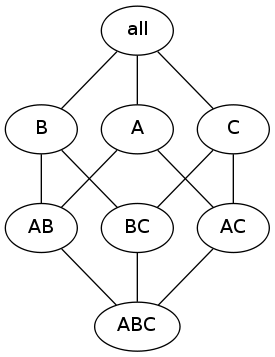
\includegraphics[scale=0.5]{dm0201.png} % scale指定缩放
% 				\caption{第一张浮动的图片}            % 图片的标题,会自动编号
% 				\label{dm0201}                % 图片的标记,一定要加在caption后面。不然指向的是前一个插图
% 			\end{figure}
% 
% 			试试使用浮动环境插入图片,但是这样图片就不知道浮动到什么地方去了:
% 
% 			\begin{figure}[htbp]                        % 
% 				\centering                              % 图片居中	
% 				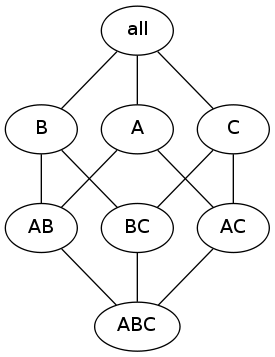
\includegraphics[scale=0.5]{dm0201.png} % scale指定缩放
% 				\caption{第二张浮动的图片}            % 图片的标题,会自动编号
% 				\label{dm0202}                % 图片的标记,一定要加在caption后面。不然指向的是前一个插图
% 			\end{figure}
% 
% 			试试使用浮动环境插入图片,但是这样图片就不知道浮动到什么地方去了:
% 
% 			\begin{figure}[htbp]                        % 
% 				\centering                              % 图片居中	
% 				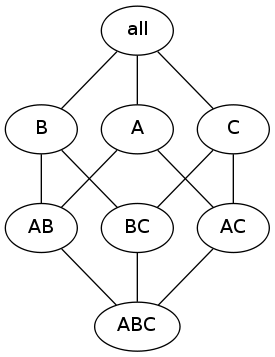
\includegraphics[scale=0.5]{dm0201.png} % scale指定缩放
% 				\caption{第三张浮动的图片}            % 图片的标题,会自动编号
% 				\label{dm0203}                % 图片的标记,一定要加在caption后面。不然指向的是前一个插图
% 			\end{figure}
% 
% 		\subsection{使用表格}
% 
% 			组表格也加上浮动环境:
% 
% 			\begin{table}[htbp]
% 				\caption{浮动环境中的三线表}
% 				\label{tab:threesome}
% 				\centering
% 				\begin{tabular}{lll}
% 					\hline
% 					操作系统 & 发行版 & 编辑器 \\
% 					\hline
% 					Windows & MikTeX & TeXnicCenter \\
% 					Unix/Linux & TeX Live & Emacs \\
% 					Mac OS & MacTeX & TeXShop \\
% 					\hline
% 				\end{tabular}
% 			\end{table}
% 

\end{document}
